\documentclass[a4paper,11pt]{article}

\usepackage[margin=3cm]{geometry}


\usepackage{graphicx}
\usepackage{subcaption}
\usepackage[colorlinks,allcolors=violet]{hyperref}
\usepackage{url}
\usepackage[dutch]{babel}



% https://tex.stackexchange.com/questions/94032/fancy-tables-in-latex
\usepackage[table]{xcolor}
\usepackage{booktabs}

\usepackage[utf8]{inputenc}

% https://tex.stackexchange.com/questions/664/why-should-i-use-usepackaget1fontenc


\newcommand{\note}[1]{{\colorbox{yellow!40!white}{#1}}}
\newcommand{\exampletext}[1]{{\color{blue!60!black}#1}}

\begin{document}

\noindent
\colorbox[HTML]{52BDEC}{\bfseries\parbox{\textwidth}{\centering\large
  --- Report P\&O CW 2019--2020 Task ST2.2 ---
}}
\\[-1mm]
\colorbox[HTML]{00407A}{\bfseries\color{white}\parbox{\textwidth}{
  Department of Computer Science -- KU Leuven
  \hfill
  \today
}}
\\

\smallskip

\noindent
\begin{tabular}{*4l}
\toprule
\multicolumn{2}{l}{\large\textbf{Team 12}} \\
\midrule
Martijn Debeuf &  22h\\ % fill in the time spend on this task per team member who worked on it
Toon Sauvillers &  22h\\
Seppe Van Steenbergen & 11h\\
\bottomrule
\hline
\end{tabular}\\

\noindent
{\color[HTML]{52BDEC} \rule{\linewidth}{1mm} }

\tableofcontents
\newpage
\section{Inleiding}\label{sec:inleiding}
	Het vorige verslag behandelde de kleurdetectie, met focus op de te herkennen kleur en de invloeden van omgevingsfactoren. Bij het herkennen van kleuren spelen oneffenheden in de foto's ook een rol, het verslag doet hiernaar verder onderzoek. Een foto is onderhevig aan verschillende factoren; Zo zal een artificiële intelligentie, die nu vaak standaard is ingebouwd in smartphones, de foto al bewerken. Lichtinval, een ander scherm of zelfs een vuil scherm, maakt dat de kleuren niet egaal worden weergegeven.

In sectie \ref{sec:achtergrond} komen verscheidene filters aan bod die de oneffenheden en ruwheden in een foto kunnen reduceren. Het zijn deze filters waar het onderzoek zich op focust. Op welke manier doen ze dit, hoe zijn deze geïmplementeerd... Vervolgens diept het verslag de toegepaste methode uit, waarna het meer uitleg geeft over de bevindingen van dit onderzoek. Een eerste zeer belangrijke factor is de tijdsconsumptie van de filter. Weegt de toeneming van uitvoeringstijd op tegen de verbetering van het resultaat? Daarnaast kan gekeken worden naar foto's die initieel niet correct werden gedetecteerd. Zorgt het toepassen van een filter ervoor dat deze wel correct wordt gedetecteerd? Welke filter geeft dan het beste resultaat? Zorgt het aanpassen van de kerngrootte voor betere detectie, en heeft dit effect op de uitvoeringstijd? Ten slotte wordt gekeken of er bevindingen toepasbaar zijn binnen het project.

\section{Achtergrond}\label{sec:achtergrond}
	Er bestaat natuurlijk een breed gamma aan fotofilters. De benodigde code voor dit onderzoek is geschreven in Python. Daarom is gekozen om vier filters uit de bibliotheek van OpenCV te gebruiken (zie sectie \ref{sec:methode}).  Een eerste toegepaste filter is de \textit{Gaussian Blur}, gevolgd door \textit{Median Blur} en \textit{Mean Blur}. Deze methodes kijken naar de pixels rond een centrale pixel om zijn kleurwaarde te bepalen. Ten slotte is er ook een minder gekende ontruismethode gebruikt namelijk de \textit{Fast Non-Local Mean Denoising}. Deze werkt anders dan de eerste drie, zie sectie \ref{subsec:fnlmd}.

\subsection{Methodes met kernelgrootte}
De volgende methodes maken gebruik van een kernelgrootte, concreet betekend dit dat het algoritme gaat kijken naar een aantal rondomliggende pixels om de nieuwe kleurwaarde te bepalen. Bij een kernelgrootte van drie zal er een vierkant met zijde drie rond de pixel getrokken worden. Elk algoritme gaat deze pixels anders interpreteren om een nieuwe waarde toe te kennen.
\subsubsection{Gaussian Blur}
De {\it Gaussian Blur} gaat kijken naar de omliggende pixels. Degenen die verder liggen, zullen minder invloed hebben dan degenen die dichterbij liggen. Een pure {\it Gaussian Blur} zou naar alle omliggende pixels kijken, ze gaan namelijk allemaal een bijdrage leveren. Door de zware berekeningen die hiermee gepaard gaan, kijkt deze blur enkel naar de omliggende pixels binnenin de door de kernelgrootte gedefinieerde omgeving. \cite{gaussianBlur}

\subsubsection{Median Blur}
Binnen de kern sorteert dit algortime de pixels van klein naar groot, vervolgens wordt de middelste waarde (mediaan) geselecteerd. De kleur van de centrale pixel van de kernel wordt dan op deze waarde geplaatst.

\subsubsection{Mean Blur}
Hier gebeurt hetzelfde als bij de {\it Median Blur} enkel neemt het algoritme hier het gemiddelde in plaats van de mediaan.

\subsection{Fast Non-Local Mean Denoising}
\label{subsec:fnlmd}
Aan  de hand van de kern worden binnen de afbeelding gelijkende kernels gezocht. Gelijkende kernen worden bij elkaar geplaatst. Van elk van deze groepen wordt dan het gemiddelde bepaald. Daarna wordt elke pixel in elke kern binnen die groep op de gemiddelde waarde geplaatst. \cite{fastExplanation} %Alle gebruikte filters bespreken

\section{Methode}\label{sec:methode}
	Verschillende componenten zijn nodig om kleuren te vergelijken. Als eerste wordt de kleur bijgehouden die op de foto staat. Daarnaast is ook de herkende kleur belangrijk. Zowel voor HSL als voor RGB kijkt het algoritme naar de kleurafstand. Bij RGB is dit de Euclidische kleurafstand. 
$$ \mid RGB \mid = \sqrt{(R_1 - R_2)^2 + (G_1 - G_2)^2 + (B_1 - B_2)^2}$$
De methode vergelijkt zo elke pixel met de ``{\it perfecte}'', te detecteren kleuren. De gedetecteerde kleur zal deze zijn met kleinste afstand tot de pixel. Op dezelfde manier zal ook HSL werken. Deze zal echter enkel kijken naar de hue-waarde, voor zwart en wit kijkt het algoritme naar de lichtheid. In tabel \ref{tab:kleuren}  staan de genomen waarden van de ``{\it perfecte}'' kleuren.

\begin{center}
\begin{table}
\label{tab:kleuren}
\centering
\begin{tabular}{ | l | c | c | }
\hline
Kleur & [R, G, B] & Hue \\
\hline
Rood & [255, 0, 0] & 0 en 360 \\
Groen & [0, 255, 0] & 120 \\
Blauw & [0, 0, 255] & 240 \\
Geel & [128, 128, 0] & 60 \\
Cyaan & [0, 128, 128] & 180 \\
Magenta & [128, 0, 128] & 300 \\
Wit & [255, 255, 255] & $L <= 10$ \\
Zwart & [0, 0, 0]] & $L >= 90$ \\
\hline
\end{tabular}
\caption{De RGB en hue waarden van de ``{\it perfecte}'' kleuren.}
\end{table}
\end{center}

Een database houdt de waarden van alle getrokken foto's bij. Het onderzoek gebruikt de verschillende eigenschappen van deze foto's. De bijgehouden eigenschappen zijn: gedetecteerde kleur, dekking van de gedetecteerde kleur, alsook de dekking van de verwachte kleur, afstand van de perfecte tot de gedetecteerde kleur, grootte van omgeving rond het scherm, soort lichtinval en de helderheid van het getrokken scherm.

\section{Bevindingen}\label{sec:bevindingen}
	In dit deel bekijkt het verslag of het al dan niet interessant is om de afbeeldingen te filteren. De eerste belangrijke indicator was tijdsconsumptie. Ook de filters onderling zijn vergelijkbaar met betrekking tot de herkenning van de kleur. Vervolgens kan gekeken worden of de kern grootte een invloed heeft op de resultaten. Ten slotte gaat het verslag na of filteren effectief het detecteren van de kleur positief beïnvloed. 

	\subsection{Tijdsconsumptie}\label{subsec:tijd}
		Wanneer gekeken wordt naar figuur \ref{fig:tijd} valt meteen op dat \textit{Fast Non-Local Mean Denoising} voor om het even welke kern grootte niet echt efficiënt is. Dit kon alreeds verwacht worden door de manier waarop deze methode te werk gaat. De waarde blijft nagenoeg constant geacht de kern grootte maar is trager met een orde van grootte 3 ten opzichte van de andere filters. Om deze reden zal deze filter al zeker niet opgenomen worden in het project. 

\begin{figure}[h!]
    \centering
    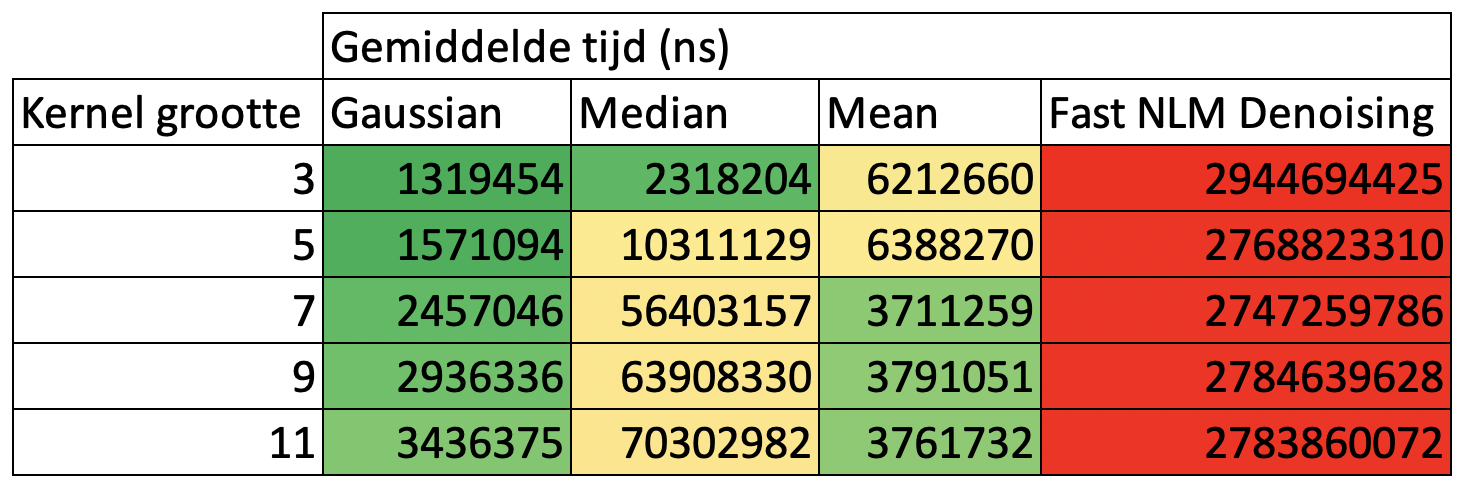
\includegraphics[scale=0.5]{img/tijdsconsumptie}
    \caption{Gemiddelde tijd nodig om filter op afbeelding toe te passen.}
    \label{fig:tijd}
\end{figure}

Voor de andere filters kunnen hun individuele tijdsgrafieken \ref{fig:tijdsgrafieken} van dichterbij bekeken worden. 
Bij de \textit{Gaussian filter} is een duidelijk lineair verband tussen kerngrootte en tijdsconsumptie zichtbaar. Dit wordt bevestigd door de determinatiecoëfficiënt van 97,85 procent van de lineaire trendlijn. 


Verder zijn er nog twee opvallende zaken. Enerzijds zorgt een grotere kern ervoor dat de \textit{Median filter} veel meer tijd nodig heeft. De reden hiervoor is dat hoe groter de kern, hoe meer elementen pixelwaarden gesorteerd moeten worden van van klein naar groot.

Bij de \textit{Mean filter} houden de waarden er nagenoeg constante waarde. Rond kern grootte 6 gebeurt een sprong in uitvoeringstijd. 
WHY??????????????????????????

 \begin{figure}[h!]
  \centering
  \begin{subfigure}{0.4\linewidth}
    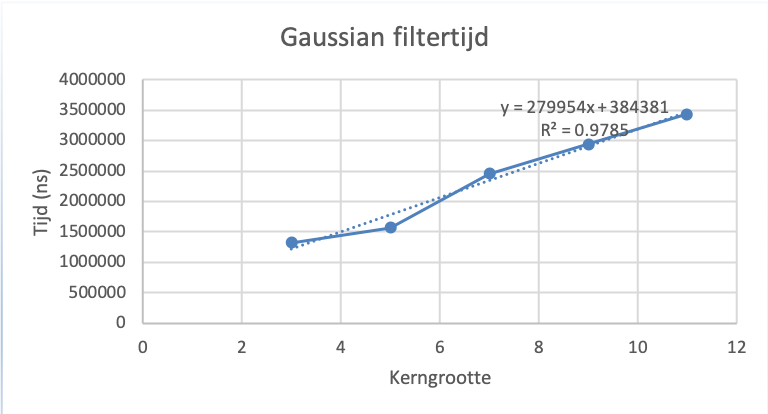
\includegraphics[width=\linewidth]{img/gaussiantijd}
  \end{subfigure}
  \begin{subfigure}{0.4\linewidth}
    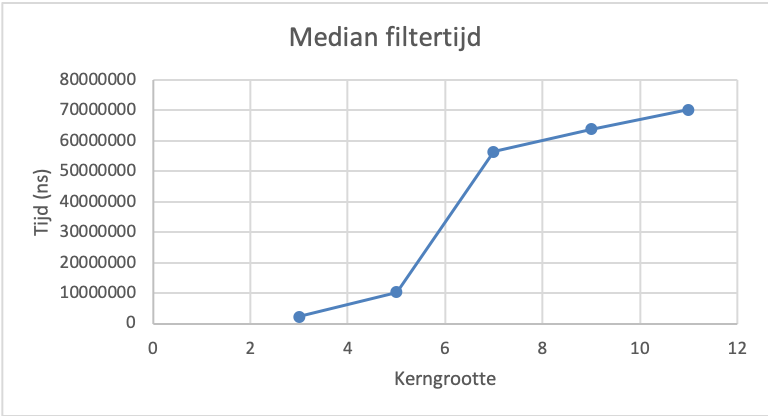
\includegraphics[width=\linewidth]{img/mediantijd}
  \end{subfigure}
  \begin{subfigure}{0.4\linewidth}
    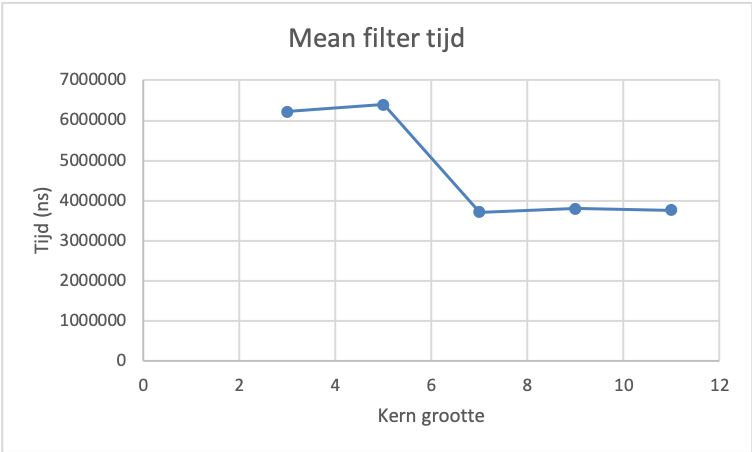
\includegraphics[width=\linewidth]{img/meantijd}
  \end{subfigure}
  \caption{Tijdsgrafieken voor de verschillende filters}
  \label{fig:tijdsgrafieken}
\end{figure}

Wanneer naar de tijdscomponent gekeken wordt geven \textit{Gaussian en Median filter} de beste resultaten. 
Op basis van tijd wordt de laatste methode al afgeschreven. 




	\subsection{Juiste herkenning}\label{subsec:juisteherkenning}
		Vervolgens bekijkt het verslag of het toepassen van een filter op een onjuist gedetecteerde foto, een al dan niet positief effect heeft.
Hiervoor maakt het onderzoek een onderscheid tussen afbeeldingen die initieel juist of initieel fout zijn gedetecteerd. 
In figuur \ref{fig:initieelfout} worden de proporties weergegeven die minder scoren na het toepassen van een filter op een initieel fout gedetecteerde afbeelding. Dit geeft dus het percentage foto's weer die slechter scoort na het filteren ervan.

\begin{figure}[h!]
  \includegraphics[width=\linewidth]{img/initieelFout}
  \caption{Proportie slechter gedetecteerde foto's na foute initiële detectie.}
  \label{fig:initieelfout}
\end{figure}

Het is opmerkelijk hoe dicht alle waarden bij elkaar liggen. Ze leunen allen zeer dicht aan tegen de $100\%$. Dit wil zeggen dat de filters de resultaten enkel verslechteren bij een al fout gedetecteerde foto. Afbeeldingen die initieel slecht scoren zullen na de filtering geen beter, tot fouter resultaat opleveren. 

Daarnaast zijn er degene die initieel juist gedetecteerd zijn. Uit figuur \ref{fig:initieeljuist} wordt al snel duidelijk dat er hier een verband is met kerngrootte. Indien de kerngrootte zeven à negen bedraagt, zullen alle afbeeldingen een hogere score hebben en dit bij alle geteste filters. Bij een grootte van drie zal ongeveer acht procent van de foto's een hogere score hebben. Kernen van grootte vijf en zeven zorgen voor een middelmaat van respectievelijk om en bij de 40 en 63 procent. Tussen de filters onderling zijn bij gelijke kerngroottes geen significante verschillen op te merken, de waarden zijn zo goed als gelijk. Het slechtere resultaat bij een kerngrootte van 11 is te wijten aan een te grote verspreiding van de oneffenheden.

Deze resultaten wijzen erop dat gebruik van filters bij de herkenning in {\it ScreenCaster} geen meerwaarde zullen hebben. Bij een foute detectie verbeteren de filters niets en bij een juiste detectie is er nog kans op een slechter resultaat.

\begin{figure}[h!]
  \includegraphics[width=\linewidth]{img/initieeljuist}
  \caption{Proportie slechter gedetecteerde foto's na foute initiële detectie.}
  \label{fig:initieeljuist}
\end{figure}
	\subsection{Gefilterd en ongefilterd} \label{subsec:gefilterd en ongefilterd}
		Om het uiteindelijke oordeel te vellen of filteren al dan niet een verbeterende factor kan zijn binnen het project, doet het verslag nog een laatste vergelijking. Namelijk kijken naar het verschil in juist gedetecteerde afbeeldingen per gebruikte methode alsook zonder het gebruik van een filter.

\begin{figure}[h!]
  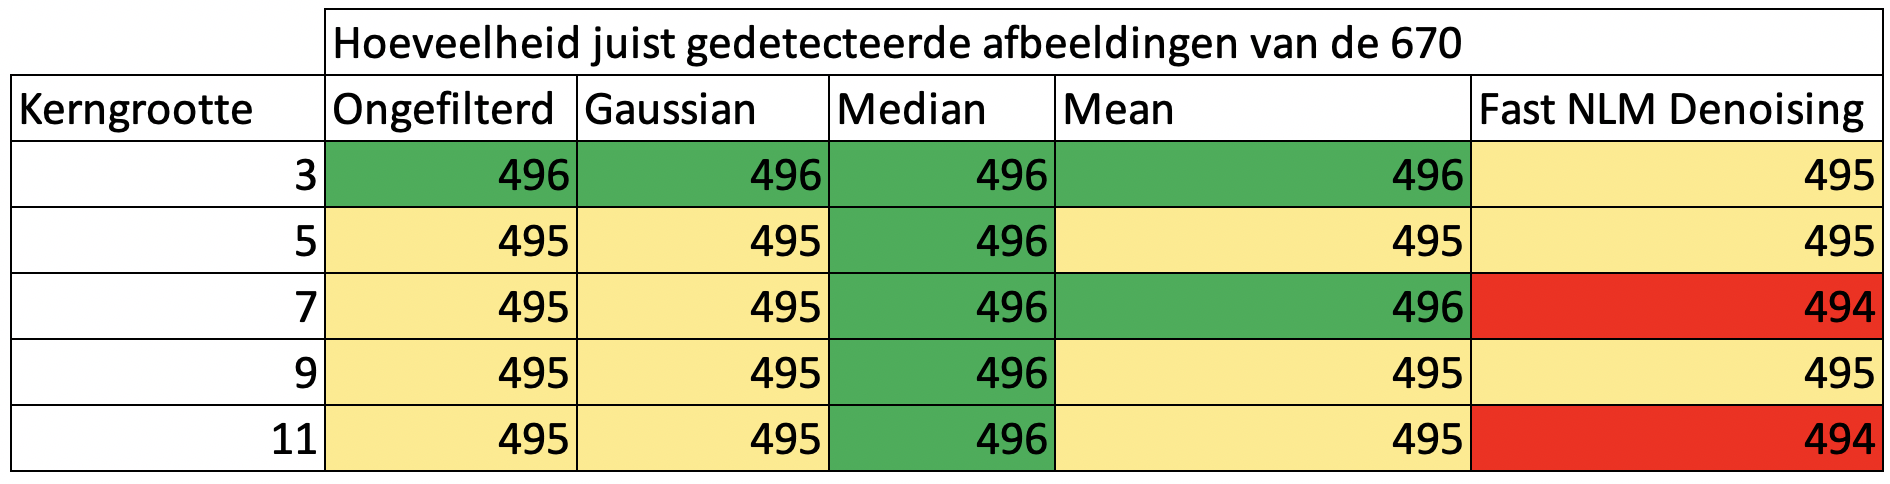
\includegraphics[width=\linewidth]{img/filternofilter}
  \caption{Aantal juist gedetecteerde foto's van de 670, gegeven de gebruikte filter.}
  \label{fig:filternofilter}
\end{figure}

Ook hier zijn de waarden nagenoeg gelijk, van de 670 afbeelding worden er bij elke toegepaste filter en gebruikte kerngrootte gemiddeld 495 correct gedetecteerd. Dit wijkt slechts af met maximaal één. Hieruit volgt alweer dat een filter toepassen nagenoeg geen effect heeft op het detecteren van de kleuren. JUIST GEDETECTEERD, MISSCHIEN OOK IN PROCENTEN ZETTEN!!!

\section{Besluit}\label{sec:besluit}
	 
Uit de bevindingen is gebleken dat de interpretatie van kleur sterk afhankelijk is van de manier waarop kleur wordt voorgesteld en de omgevingsfactoren die hierbij aanwezig zijn. Enerzijds speelt de kleurruimte waarin een kleur wordt voorgesteld een grote rol bij de detectie. Van de verschillende kleurruimten die bekeken zijn, is er niet een die eenduidig beter is dan de andere. Beiden hebben hun voordelen, zo is HSL beter voor de detectie van alle kleuren dan RGB. Maar de detectieratio van zwart en wit is dan wel weer aannoemelijk beter in RGB dan in HSL.  Anderzijds spelen omgevingsfactoren ook een belangrijke rol bij de detectie van de kleuren. Hiervoor werd gekeken naar zowel de omgeving, de lichtinval en de helderheid van het scherm. De belangrijkste bevindingen hierbij hebben te maken met de lichtinval en de omgeving. Door lichtinval komt er bij artificieel licht extra rood in de kleuren door de rode schijn die het licht achterlaat. Hoe groter de omgeving, hoe meer de kleuren fout gedetecteerd gaan worden. Dit is te wijten aan het feit dat de camera hierbij op de omgeving gaat focussen in plaats van op het scherm. Tot slot is ook gebleken dat helderheid geen groot effect heeft op de detectie.
	
	\subsection{Toepassingen op het project}\label{subsec:toepassingen}
		Voor het detectiealgoritme kan het best gebruik gemaakt worden van de HSL kleurruimte zoals nu al het geval is. Maar voor het identificatiealgoritme waarbij wit en zwart gebruikt wordt, zou beter overgeschakeld worden naar een algoritme dat gebruik maakt van de RGB kleurruimte.

De keuze voor de drie kleuren die weergegeven worden op het detectiescherm valt op rood, groen en blauw. Deze drie kleuren hebben een grote detectieratio en de omgevingsfactoren hebben het minste invloed op deze kleuren.

Aan de hand van de bevindingen rondom omgeving moeten foto's zo dicht mogelijk getrokken worden bij de opstelling zodat de omgeving minimaal is. Natuurlijk moet wel heel de opstelling in de foto passen.



\medskip

\bibliographystyle{unsrt}
\bibliography{Bibliography}

\end{document}